\documentclass[aspectratio=169]{beamer}

% ── Theme ────────────────────────────────────────────────────────────────────
\usetheme{Boadilla}
\usecolortheme{default}
\setbeamertemplate{navigation symbols}{}
\setbeamertemplate{footline}[frame number]

% ── Packages ─────────────────────────────────────────────────────────────────
\usepackage{graphicx}
\usepackage{booktabs}
\usepackage{colortbl}
\usepackage{xcolor}
\usepackage{tikz}
\usepackage{pgfpages}
\usetikzlibrary{shapes.geometric, arrows.meta, positioning, fit, backgrounds, calc}

% To show speaker notes on a second screen, uncomment the next line:
% \setbeameroption{show notes on second screen=right}

% ── Colors ───────────────────────────────────────────────────────────────────
\definecolor{rfgreen}{RGB}{0,153,76}
\definecolor{phblue}{RGB}{0,56,168}
\definecolor{lightblue}{RGB}{220,235,255}
\definecolor{lightgreen}{RGB}{210,245,225}

% ── Image paths (repo-relative) ───────────────────────────────────────────────
% Required images NOT in the repo (source externally and place in images/):
%   images/tractor_ph_rice_field.jpg  — full-bleed tractor in Philippine rice field
%   images/combine_harvester.jpg      — large combine harvester
%   images/water_pump_stationary.jpg  — small stationary water pump
\graphicspath{
  {../../Mini-Project/Agricultural Machinery Inventory from ABEMIS/Regression Parameters Output V3/}
  {../../Mini-Project/Agricultural Machinery Inventory from ABEMIS/Analytics Output V2/}
  {../Agricultural Machinery Inventory from ABEMIS/Regression Parameters Output V3/}
  {../Agricultural Machinery Inventory from ABEMIS/Analytics Output V2/}
  {images/}
}

% ── Title metadata ────────────────────────────────────────────────────────────
\title[Fuel Estimation ML]{%
  Pilot Machine Learning Model for\\
  Fuel Requirement Estimation\\
  in Agricultural Mechanization%
}
\author{Ronald Melvin R.\ Rosas \and Marcus Rafael Tiongson}
\institute{AI 201 --- University of the Philippines, Diliman}
\date{}

% ─────────────────────────────────────────────────────────────────────────────
\begin{document}

% ── Slide 1: Title & Hook ────────────────────────────────────────────────────
{%
\IfFileExists{images/farmersKYC.jpg}{%
  \usebackgroundtemplate{%
    \begin{tikzpicture}[remember picture,overlay]

      % Background image
      \node[inner sep=0pt] (bgimg)
      at (current page.center)
      {
        \includegraphics[
          width=\paperwidth,
          height=\paperheight
        ]{farmersKYC.jpg}
      };

      % Dark overlay
      \fill[
        black,
        opacity=0.75
      ]
      (current page.south west)
      rectangle
      (current page.north east);

    \end{tikzpicture}
  }%
}{}

\begin{frame}[plain]

  \vspace{2.2cm}

  \centering

  % Main Title
  {\color{white}\LARGE\bfseries
    Pilot Machine Learning Model for\\[0.4em]
    Fuel Requirement Estimation\\[0.4em]
    in Agricultural Mechanization
  }

  \vspace{1.2em}

  % Authors
  {\color{white}\normalsize
    Ronald Melvin R.\ Rosas \quad|\quad Marcus Rafael Tiongson
  }

  \vspace{0.3em}

  % Affiliation
  {\color{white}\small
    AI 201 --- University of the Philippines Diliman
  }

  % ── Photo Credit Overlay ───────────────────────────────────────────────
  \begin{tikzpicture}[remember picture,overlay]

    \node[
      anchor=south west,
      xshift=0.45cm,
      yshift=0.30cm,
      fill=black,
      fill opacity=0.72,
      text opacity=1,
      rounded corners=3pt,
      inner sep=5pt
    ]
    at (current page.south west)
    {
      \parbox{0.74\paperwidth}{
        \color{white}\scriptsize\textit{
        Photo credit: DA Region VII --- Conduct of KYC verification of farmers and fisherfolk beneficiaries of Fuel Assistance to Farmers and Fisherfolk.
        }
      }
    };

  \end{tikzpicture}

  % Speaker Notes
  \note{
  Introduce the core thesis immediately. We are moving from static,
  outdated engineering estimates to dynamic, data-driven machine learning.
  This pilot shows that a Random Forest trained on AMTEC test data reaches
  R\textsuperscript{2} = 0.916 and immediately scores 172,265 machines
  across the national ABEMIS inventory.
  }

\end{frame}
}



% ── Slide 2: Philippine Agricultural Mechanization Context ──────────────────
\begin{frame}{Agricultural Mechanization in the Philippine Context}

\centering

% Main diagram/image
\IfFileExists{images/Philippine Agricultural Mechanization Context Diagram.png}{%
    \includegraphics[
        width=0.96\linewidth,
        height=0.72\textheight,
        keepaspectratio
    ]{images/Philippine Agricultural Mechanization Context Diagram.png}
}{%
    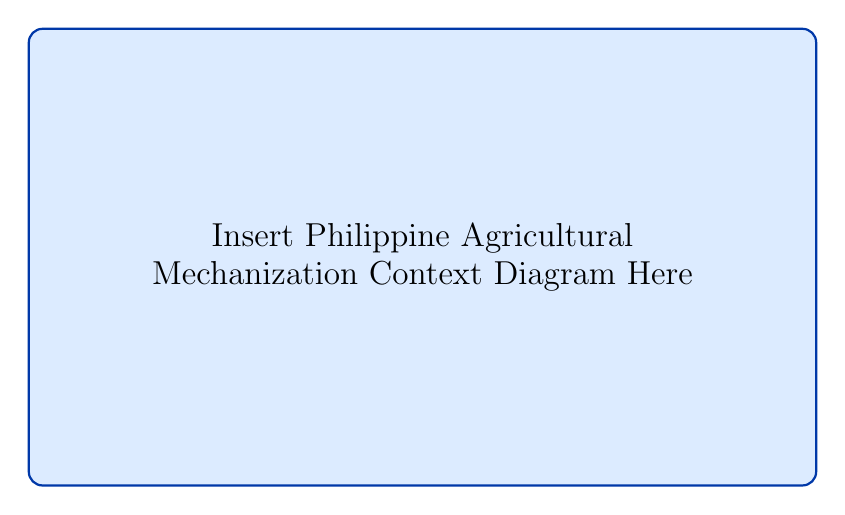
\begin{tikzpicture}

        % Placeholder box if image is missing
        \draw[
            phblue,
            thick,
            rounded corners=5pt,
            fill=lightblue
        ]
        (0,0) rectangle (10,5.8);

        \node[
            align=center,
            font=\large
        ]
        at (5,2.9)
        {
            Insert Philippine Agricultural\\
            Mechanization Context Diagram Here
        };

    \end{tikzpicture}
}

\vspace{0.45em}

% Context statement box
\begin{center}
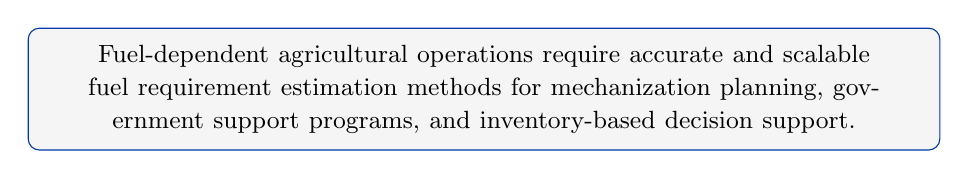
\begin{tikzpicture}
\node[
    fill=black!4,
    draw=phblue,
    rounded corners=4pt,
    inner sep=6pt,
    text width=0.92\linewidth,
    align=center
]
{
\small
Fuel-dependent agricultural operations require accurate and scalable
fuel requirement estimation methods for mechanization planning,
government support programs, and inventory-based decision support.
};
\end{tikzpicture}
\end{center}

\vspace{0.2em}

% Transition statement
{\scriptsize\textit{
However, fuel requirement estimation remains challenging because
agricultural machinery operations exhibit highly variable real-world behavior.
}}

\note{
This slide establishes the broader Philippine agricultural mechanization
context. Mechanization contributes to productivity improvement,
rural income generation, operational efficiency, and agricultural
development. Government support, machinery access, infrastructure,
and financing all influence mechanization adoption.

Because mechanized agricultural operations are fuel-dependent,
accurate fuel requirement estimation becomes important for planning,
resource allocation, and support programs. However, machinery
operations vary significantly depending on machine type, operating
conditions, field environment, and workload characteristics. This
creates challenges for traditional deterministic fuel estimation methods
and motivates the need for data-driven machine learning approaches.
}

\end{frame}






% ── Slide 3: The Data ────────────────────────────────────────────────────────
\begin{frame}{The Data: AMTEC \& ABEMIS}
  \begin{center}
  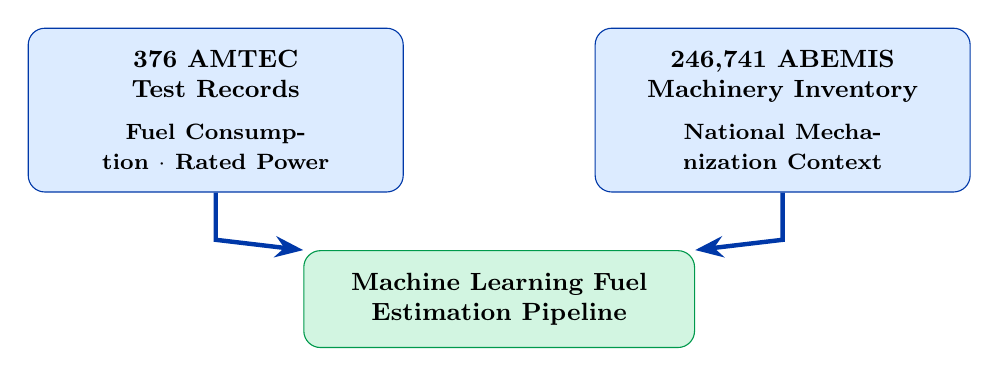
\begin{tikzpicture}[
    box/.style={rectangle, rounded corners=6pt, draw=phblue, fill=lightblue,
                text width=4.2cm, align=center, font=\small\bfseries,
                minimum height=1.6cm, inner sep=8pt},
    merge/.style={rectangle, rounded corners=6pt, draw=rfgreen, fill=lightgreen,
                  text width=4.4cm, align=center, font=\small\bfseries,
                  minimum height=1.1cm, inner sep=8pt},
    arrow/.style={-Stealth, phblue, line width=1.6pt}
  ]
    \node[box] at (-3.6, 0) (amtec)
      {\textbf{376} AMTEC\\Test Records\\[4pt]
       \footnotesize Fuel Consumption $\cdot$ Rated Power};
    \node[box] at (3.6, 0) (abemis)
      {\textbf{246{,}741} ABEMIS\\Machinery Inventory\\[4pt]
       \footnotesize National Mechanization Context};
    \node[merge] at (0, -2.4) (ml)
      {Machine Learning Fuel Estimation Pipeline};
    \draw[arrow] (amtec.south) -- ++(0,-0.6) -- ($(ml.north west)+(0,0)$);
    \draw[arrow] (abemis.south) -- ++(0,-0.6) -- ($(ml.north east)+(0,0)$);
  \end{tikzpicture}
  \end{center}
  \vspace{0.3em}
  \begin{columns}[t]
    \column{0.48\textwidth}
      \textbf{AMTEC} --- Philippine machinery testing and evaluation center, based in UPLB, providing standardized agricultural machinery performance and fuel consumption data.\\
      {\small Source: UPLB-AMTEC (1990s--2026)}
    \column{0.48\textwidth}
      \textbf{ABEMIS} --- National agricultural engineering information system of BAFE for machinery inventory, infrastructure monitoring, and mechanization decision support.\\
      {\small Coverage: all 18 Philippine regions}
  \end{columns}
  \note{Briefly establish data provenance. You took standardized, controlled test
  data from AMTEC and enriched it with massive, real-world deployment context from
  ABEMIS. The join provides regional prevalence and machinery-type distribution as
  context features for the model.}
\end{frame}

% ── Slide 4: Why Random Forest? ───────────────────────────────────────────────
\begin{frame}{The Engine: Capturing Non-Linear Physical Interactions}
  \begin{columns}[c]
    \column{0.54\textwidth}
      \centering
      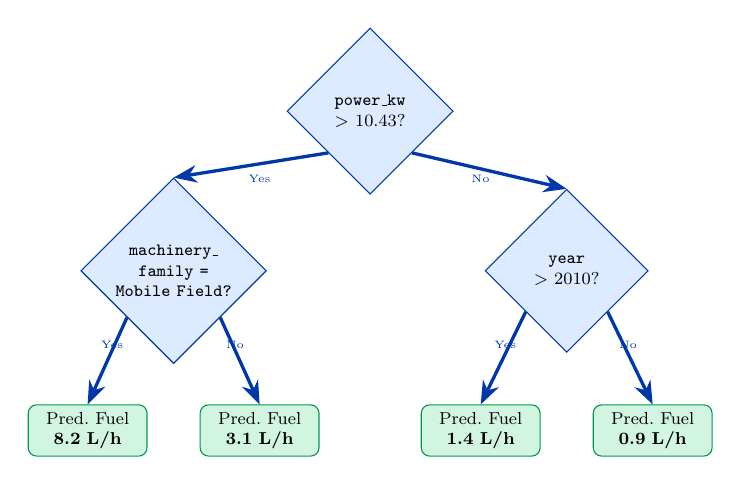
\begin{tikzpicture}[
        scale=0.78, transform shape,
        decision/.style={diamond, draw=phblue, fill=lightblue,
                         inner sep=2pt, text width=1.9cm, align=center,
                         font=\footnotesize},
        leaf/.style={rectangle, rounded corners=3pt, draw=rfgreen, fill=lightgreen,
                     text width=1.7cm, align=center, minimum height=0.75cm,
                     font=\footnotesize},
        arrow/.style={-Stealth, phblue, line width=1.2pt}
      ]
        % Nodes — manually placed
        \node[decision] (root) at (0, 0)
          {\texttt{power\_kw}\\ $>$ 10.43?};
        \node[decision] (left)  at (-3.2, -2.6)
          {\texttt{machinery\_}\\\texttt{family =}\\\texttt{Mobile Field?}};
        \node[decision] (right) at ( 3.2, -2.6)
          {\texttt{year}\\ $>$ 2010?};
        \node[leaf] (ll) at (-4.6, -5.2)
          {Pred.\ Fuel\\\textbf{8.2 L/h}};
        \node[leaf] (lr) at (-1.8, -5.2)
          {Pred.\ Fuel\\\textbf{3.1 L/h}};
        \node[leaf] (rl) at ( 1.8, -5.2)
          {Pred.\ Fuel\\\textbf{1.4 L/h}};
        \node[leaf] (rr) at ( 4.6, -5.2)
          {Pred.\ Fuel\\\textbf{0.9 L/h}};
        % Edges
        \draw[arrow] (root.south west) -- (left.north);
        \draw[arrow] (root.south east) -- (right.north);
        \draw[arrow] (left.south west)  -- (ll.north);
        \draw[arrow] (left.south east)  -- (lr.north);
        \draw[arrow] (right.south west) -- (rl.north);
        \draw[arrow] (right.south east) -- (rr.north);
        % Edge labels
        \node[font=\tiny, phblue] at (-1.8, -1.1) {Yes};
        \node[font=\tiny, phblue] at ( 1.8, -1.1) {No};
        \node[font=\tiny, phblue] at (-4.2, -3.8) {Yes};
        \node[font=\tiny, phblue] at (-2.2, -3.8) {No};
        \node[font=\tiny, phblue] at ( 2.2, -3.8) {Yes};
        \node[font=\tiny, phblue] at ( 4.2, -3.8) {No};
      \end{tikzpicture}
    \column{0.44\textwidth}
      \textbf{Why not OLS?}
      \begin{itemize}\setlength\itemsep{0.5em}
        \item Power and fuel do \emph{not} scale linearly across machine types
        \item Each tree partitions the feature space differently
        \item 300 trees average out variance — robust predictions
        \item No manual feature crossing required
      \end{itemize}
      \vspace{0.7em}
      {\small$R^2_{\text{RF}} = 0.916$ \quad vs.\quad $R^2_{\text{OLS}} = 0.704$}
  \end{columns}
  \note{This is the primary methodology. Engine power and machinery type don't scale
  linearly. Random Forest was explicitly chosen because its ensemble of decision trees
  inherently captures these complex, non-linear interactions without requiring manual
  feature crossing.}
\end{frame}

% ── Slide 5: Results ─────────────────────────────────────────────────────────
\begin{frame}{Random Forest vs.\ OLS Baseline ($n_{\text{test}}=76$)}
  \centering
  \vspace{0.3em}
  \begin{tabular}{lccc}
    \toprule
    \textbf{Model}
      & \textbf{R\textsuperscript{2}}
      & \textbf{MAE (L/h)}
      & \textbf{RMSE (L/h)} \\
    \midrule
    OLS Global Linear         & 0.704 & 1.882 & 2.875 \\
    OLS Hierarchical Fallback & 0.703 & 1.879 & 2.879 \\
    \rowcolor{rfgreen!25}
    \textcolor{rfgreen}{\textbf{Random Forest}}
      & \textcolor{rfgreen}{\textbf{0.916}}
      & \textcolor{rfgreen}{\textbf{0.950}}
      & \textcolor{rfgreen}{\textbf{1.534}} \\
    \bottomrule
  \end{tabular}

  \vspace{1.0em}
  \begin{columns}[c]
    \column{0.3\textwidth}\centering
      {\color{rfgreen}\Huge\bfseries $+$30\%}\\[2pt]{\small better $R^2$}
    \column{0.3\textwidth}\centering
      {\color{rfgreen}\Huge\bfseries $2\times$}\\[2pt]{\small lower MAE}
    \column{0.3\textwidth}\centering
      {\color{rfgreen}\Huge\bfseries $2\times$}\\[2pt]{\small lower RMSE}
  \end{columns}
  \note{Let the numbers speak. The RF model achieves R² = 0.916 with MAE = 0.95 L/h.
  It substantially outperforms the hierarchical OLS fallback because it adapts to the
  feature variances that linear models smooth over.}
\end{frame}

% ── Slide 5b: OLS Diagnostics — Global (All Machinery) ───────────────────────
\begin{frame}{OLS Diagnostics --- Global (All Machinery)}
  \begin{columns}[c]
    \column{0.48\textwidth}
      \centering
      \includegraphics[width=\linewidth,height=0.72\textheight,keepaspectratio]%
        {GLOBAL_ALL_MACHINERY_FINAL_quadratic_residuals_vs_fitted.png}
      {\scriptsize Residuals vs.\ fitted}
    \column{0.48\textwidth}
      \centering
      \includegraphics[width=\linewidth,height=0.72\textheight,keepaspectratio]%
        {GLOBAL_ALL_MACHINERY_FINAL_quadratic_qqplot.png}
      {\scriptsize Q--Q plot}
  \end{columns}
  \vspace{0.3em}
  {\footnotesize Residuals fan out at the high-power tail and the Q--Q deviates in the upper quantiles --- the global quadratic OLS underfits heavy mobile machinery, motivating the per-family fallback and the move to Random Forest.}
  \note{The global OLS fit shows clear heteroscedasticity at high power and tail
  departure from normality. This is the empirical reason the hierarchical fallback
  and the non-parametric RF outperform a single linear model.}
\end{frame}

% ── Slide 5c: OLS Diagnostics — Mobile Field Machinery ───────────────────────
\begin{frame}{OLS Diagnostics --- Mobile Field Machinery}
  \begin{columns}[c]
    \column{0.48\textwidth}
      \centering
      \includegraphics[width=\linewidth,height=0.72\textheight,keepaspectratio]%
        {MACHINERY_FAMILY_Mobile_Field_Machinery_FINAL_quadratic_residuals_vs_fitted.png}
      {\scriptsize Residuals vs.\ fitted}
    \column{0.48\textwidth}
      \centering
      \includegraphics[width=\linewidth,height=0.72\textheight,keepaspectratio]%
        {MACHINERY_FAMILY_Mobile_Field_Machinery_FINAL_quadratic_qqplot.png}
      {\scriptsize Q--Q plot}
  \end{columns}
  \vspace{0.3em}
  {\footnotesize Within the Mobile Field family (tractors, tillers) the quadratic fit is markedly tighter --- residuals are more symmetric and the Q--Q tracks normal across most of the range, validating the per-family scope as the most useful OLS slice.}
  \note{Tractors and tillers are the cleanest OLS slice. Once we restrict to one
  physical family, the quadratic in power\_kw recovers most of the variance.}
\end{frame}

% ── Slide 5d: OLS Diagnostics — Harvest Machinery ────────────────────────────
\begin{frame}{OLS Diagnostics --- Harvest Machinery}
  \begin{columns}[c]
    \column{0.48\textwidth}
      \centering
      \includegraphics[width=\linewidth,height=0.72\textheight,keepaspectratio]%
        {MACHINERY_FAMILY_Harvest_Machinery_FINAL_quadratic_residuals_vs_fitted.png}
      {\scriptsize Residuals vs.\ fitted}
    \column{0.48\textwidth}
      \centering
      \includegraphics[width=\linewidth,height=0.72\textheight,keepaspectratio]%
        {MACHINERY_FAMILY_Harvest_Machinery_FINAL_quadratic_qqplot.png}
      {\scriptsize Q--Q plot}
  \end{columns}
  \vspace{0.3em}
  {\footnotesize Harvest machinery (combines, reapers) holds a serviceable quadratic shape but with a heavier upper-quantile Q--Q tail than Mobile Field --- a residual non-linearity that Random Forest captures without needing manual feature engineering.}
  \note{Combines and reapers show more heavy-tailed residuals than tractors.
  This is exactly the structure that the non-parametric RF picks up.}
\end{frame}

% ── Section Divider: Why trust it? ───────────────────────────────────────────
{%
\IfFileExists{images/tractor_ph_rice_field.jpg}{%
  \usebackgroundtemplate{%
    \begin{tikzpicture}
      \node[inner sep=0pt] (bgimg) at (0,0)
        {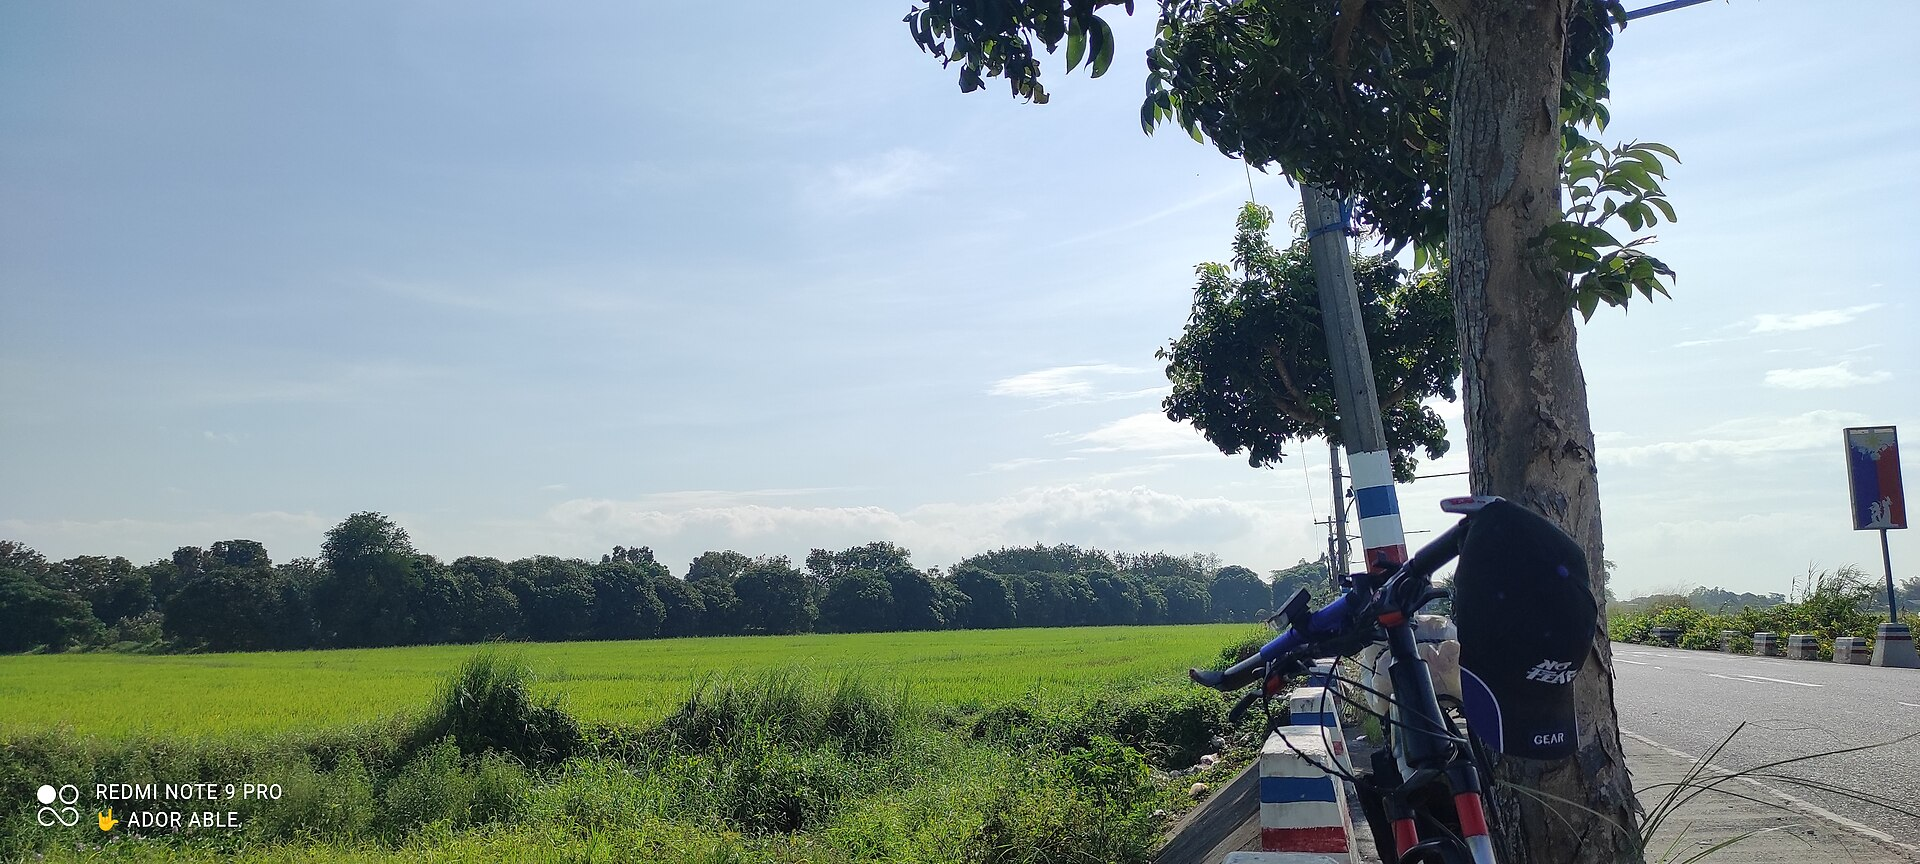
\includegraphics[width=\paperwidth,height=\paperheight]{tractor_ph_rice_field.jpg}};
      \fill[black,opacity=0.55] (bgimg.south west) rectangle (bgimg.north east);
    \end{tikzpicture}}%
}{}
\begin{frame}[plain]
  \vspace{2.4cm}
  \centering
  {\color{white}\Huge\bfseries
    But why does the model\\[0.3em]
    trust these predictions?}\\[1.4em]
  {\color{white!85}\large
    Opening the black box with SHAP and LIME.}
  \note{Pivot from raw metrics into interpretability. Strong R² is not enough ---
  BAFE engineers must understand why the model makes each call before they will
  trust it for national planning.}
\end{frame}
}

% ── Slide 6: SHAP Global Interpretability ────────────────────────────────────
\begin{frame}{What Drives the Model? (Validating Physics with SHAP)}
  \begin{columns}[c]
    \column{0.60\textwidth}
      \centering
      \includegraphics[width=\linewidth,height=0.76\textheight,keepaspectratio]%
        {shap_summary_bar.png}
    \column{0.38\textwidth}
      \textbf{Key finding:}\\[0.5em]
      \texttt{power\_kw} accounts for \textbf{$\sim$66.5\%} of total prediction importance.\\[0.8em]
      \texttt{year} (equipment vintage) is second at \textbf{$\sim$12.3\%}, reflecting improved combustion efficiency in newer equipment.\\[0.8em]
      ABEMIS context features contribute a combined \textbf{$\sim$9\%}, adding real but secondary value.\\[0.8em]
      {\small The model didn't memorize data --- it \emph{learned physics}.}
  \end{columns}
  \note{The model didn't just memorize data; it learned actual physics. Point out that
  power\_kw dictates ~66.5\% of the prediction importance, with year second at ~12.3\%
  capturing equipment-generation efficiency gains. This perfectly mirrors the
  established physical laws of fuel power proportionality. ABEMIS context features
  contribute a combined ~9\%, providing contextual fine-tuning.}
\end{frame}

% ── Slide 6b: SHAP Beeswarm ──────────────────────────────────────────────────
\begin{frame}{SHAP Beeswarm --- Distribution of Feature Contributions}
  \centering
  \includegraphics[width=0.92\textwidth,height=0.76\textheight,keepaspectratio]%
    {shap_summary_beeswarm.png}

  \vspace{0.3em}
  {\small Each dot is one test record; color encodes feature value (red = high, blue = low).
  High \texttt{power\_kw} consistently pushes predictions up;
  \texttt{year} contributions are bidirectional, capturing both older high-fuel
  and modern efficient cohorts.}
  \note{Where the bar chart tells you which features matter, the beeswarm tells you
  how each feature value moves the prediction. Red dots on power\_kw stretch far to the right
  --- high-power machines always raise the estimate. The year feature splits into two clusters,
  showing the vintage effect cleanly.}
\end{frame}

% ── Slide 7: LIME Local Interpretability ─────────────────────────────────────
\begin{frame}{Explaining Individual Predictions (LIME)}
  \centering
  \includegraphics[width=0.88\textwidth,height=0.72\textheight,keepaspectratio]%
    {lime_example_0.png}

  \vspace{0.4em}
  {\small LIME breaks down \emph{why} the model predicted \textbf{4.77\,L/h} for one
  specific small engine --- granular transparency that builds trust for BAFE engineers.}
  \note{Frame this around stakeholder trust. While SHAP explains the entire model,
  LIME breaks down why the model predicted 4.77 L/h for one specific small engine.
  This granular transparency is how you get BAFE engineers to actually trust and
  adopt the tool.}
\end{frame}

% ── Slide 7b: LIME — more samples (2x2 grid) ─────────────────────────────────
\begin{frame}{LIME --- More Local Explanations Across Machinery Types}
  \centering
  \begin{tabular}{cc}
    
\includegraphics[width=0.44\textwidth,keepaspectratio]{lime_example_1.png} &
    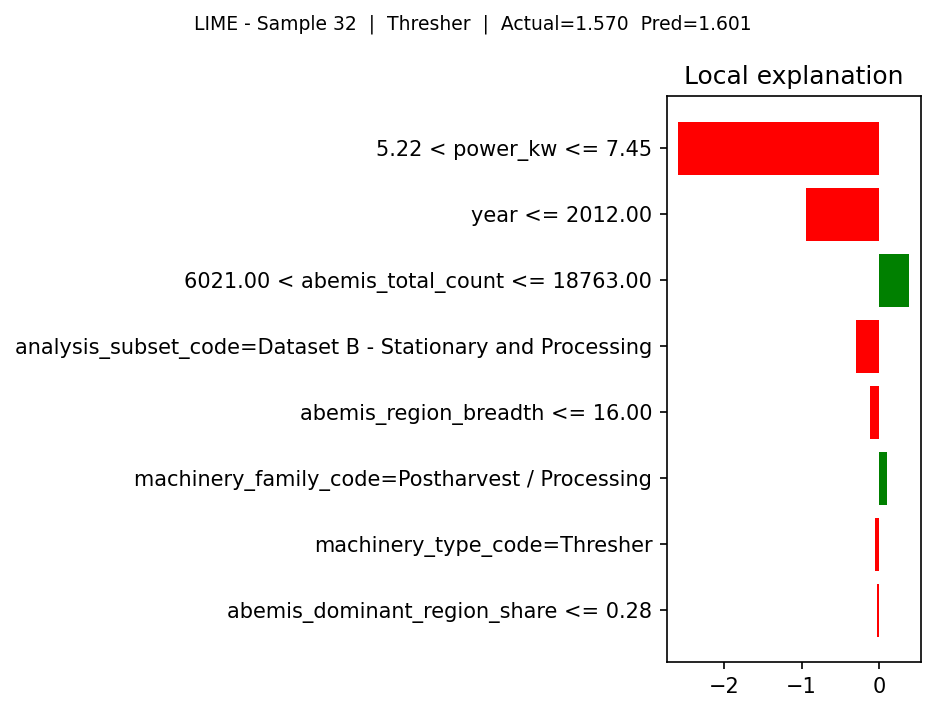
\includegraphics[width=0.44\textwidth,keepaspectratio]{lime_example_2.png} \\[0.3em]
    
\includegraphics[width=0.44\textwidth,keepaspectratio]{lime_example_3.png} &
    
\includegraphics[width=0.44\textwidth,keepaspectratio]{lime_example_4.png} \\
  \end{tabular}

  \vspace{0.2em}
  {\footnotesize Across 10 inspected records, \texttt{power\_kw} is the top
  local contributor in 9 out of 10 cases; \texttt{machinery\_type} and
  \texttt{analysis\_subset} carry the secondary adjustments, particularly
  for dryers and stationary processing equipment.}
  \note{Four LIME plots in a grid demonstrate that the single-instance view
  on the previous slide is not cherry-picked. Power dominates locally for
  almost every record; type and subset modulate the magnitude.}
\end{frame}

% ── Slide 8: National Impact ──────────────────────────────────────────────────
\begin{frame}{From Lab to National Scale}
  \begin{columns}[c]
    \column{0.50\textwidth}
      \centering
      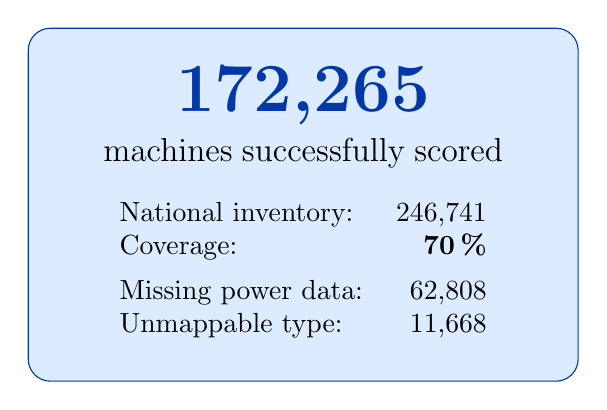
\begin{tikzpicture}
        \node[rectangle, rounded corners=8pt,
              draw=phblue, fill=lightblue,
              text width=6.0cm, align=center, inner sep=14pt] {
          {\color{phblue}\fontsize{36}{40}\selectfont\bfseries 172{,}265}\\[4pt]
          {\large machines successfully scored}\\[10pt]
          \begin{tabular}{lr}
            National inventory: & 246{,}741 \\
            Coverage:           & \textbf{70\,\%} \\[4pt]
            Missing power data: & 62{,}808 \\
            Unmappable type:    & 11{,}668 \\
          \end{tabular}
        };
      \end{tikzpicture}
    \column{0.48\textwidth}
      \textbf{Outputs per region:}
      \begin{itemize}\setlength\itemsep{0.5em}
        \item Per-record fuel estimate (L/h)
        \item Per-region aggregate demand
        \item Per-region $\times$ machinery-type breakdown
      \end{itemize}
      \vspace{0.8em}
      The unscored 30\% reflects \emph{data gaps} --- not model failure. Closing
      those gaps is part of the roadmap.
  \end{columns}
  \note{You successfully scored 70\% of the national inventory. Clarify that the
  unscored 30\% were due to raw data gaps (missing power ratings / unmappable types).
  The takeaway: this model immediately enables data-driven mechanization planning
  across all 17 regions.}
\end{frame}

% ── Section Divider: What's next? ────────────────────────────────────────────
{%
\IfFileExists{images/ph_field_aerial.jpg}{%
  \usebackgroundtemplate{%
    \begin{tikzpicture}
      \node[inner sep=0pt] (bgimg) at (0,0)
        {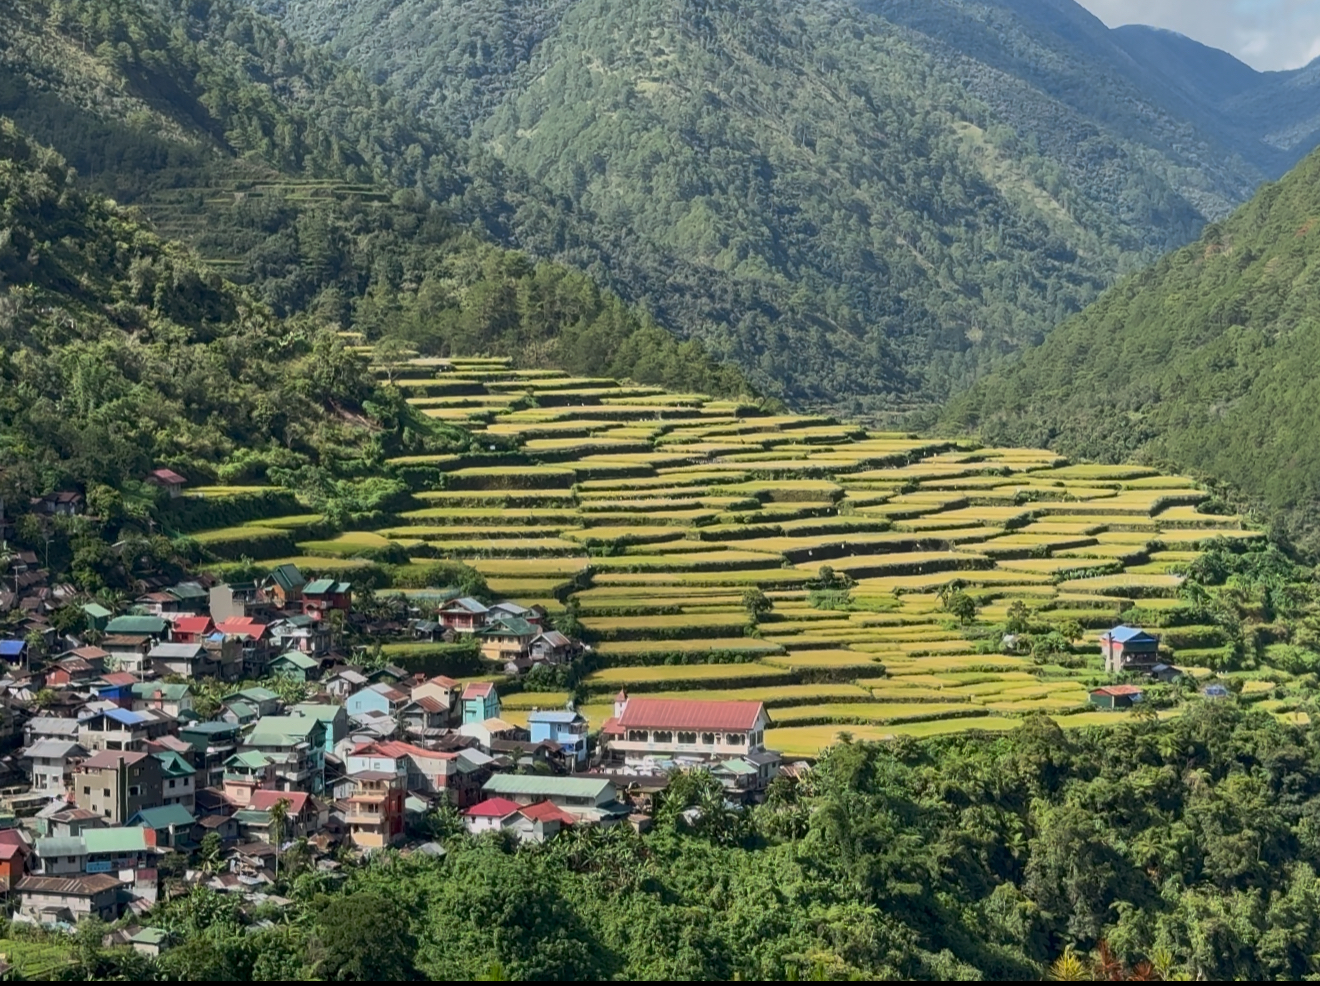
\includegraphics[width=\paperwidth,height=\paperheight]{ph_field_aerial.jpg}};
      \fill[black,opacity=0.55] (bgimg.south west) rectangle (bgimg.north east);
    \end{tikzpicture}}%
}{}
\begin{frame}[plain]
  \vspace{2.4cm}
  \centering
  {\color{white}\Huge\bfseries
    What's next?}\\[1.4em]
  {\color{white!85}\large
    Closing the data gaps. Validating in the field.}
  \note{Reset the audience visually before the roadmap. Three concrete next
  iterations: enlarge the corpus via the 3,065-PDF set; integrate the RAED
  cropping calendar; validate against in-field GPS/flow-sensor telemetry.}
\end{frame}
}


% ── Slide 9: Future Work ──────────────────────────────────────────────────────
\begin{frame}{Future Directions of the Study}

\vspace{0.4em}

\begin{center}
\small
The proposed framework may be expanded toward national-scale
fuel forecasting, seasonal planning, and data-driven mechanization support.
\end{center}

\vspace{0.8em}

\begin{columns}[c]

% ───────────────── Left Column ─────────────────
\column{0.32\textwidth}
\centering


\begin{tikzpicture}
\node[
    circle,
    draw=phblue,
    fill=lightblue,
    minimum size=1.9cm,
    font=\Large\bfseries
] {\Large$\Sigma$};
\end{tikzpicture}

\vspace{0.6em}

\textbf{National Fuel Forecasting}

\vspace{0.4em}

\small
Estimate regional and seasonal agricultural fuel demand
using national machinery inventories and operational datasets.

% ───────────────── Middle Column ─────────────────
\column{0.32\textwidth}
\centering


\begin{tikzpicture}
\node[
    circle,
    draw=phblue,
    fill=lightblue,
    minimum size=1.9cm,
    font=\Large\bfseries
] {\small calendar};
\end{tikzpicture}

\vspace{0.6em}

\textbf{Seasonal Planning}

\vspace{0.4em}

\small
Integrate cropping calendars to identify peak planting
and harvesting fuel demand periods.

% ───────────────── Right Column ─────────────────
\column{0.32\textwidth}
\centering


\begin{tikzpicture}
\node[
    circle,
    draw=phblue,
    fill=lightblue,
    minimum size=1.9cm,
    font=\Large\bfseries
] {\Large$\checkmark$};
\end{tikzpicture}

\vspace{0.6em}

\textbf{Real-World Validation}

\vspace{0.4em}

\small
Compare machine learning predictions against
actual farm-level fuel consumption observations.

\end{columns}

\vspace{1.0em}

% Bottom implication box
\begin{center}
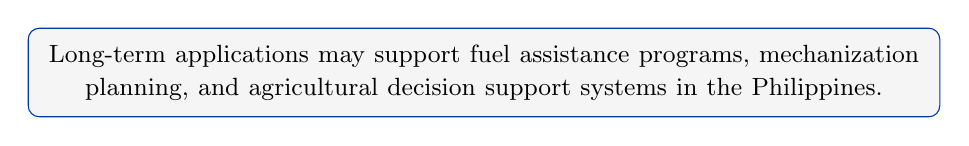
\begin{tikzpicture}
\node[
    fill=black!4,
    draw=phblue,
    rounded corners=4pt,
    inner sep=6pt,
    text width=0.92\linewidth,
    align=center
]
{
\small
Long-term applications may support fuel assistance programs,
mechanization planning, and agricultural decision support systems
in the Philippines.
};
\end{tikzpicture}
\end{center}

\note{
The long-term goal of this work extends beyond predictive modeling.
The framework may eventually support regional fuel forecasting,
seasonal agricultural planning, mechanization analytics, and
evidence-based government support programs.

Future work includes expanding operational datasets, integrating
cropping calendars to model seasonal demand behavior, and validating
predictions using real-world agricultural fuel consumption observations.
These developments may help improve large-scale mechanization planning
and agricultural decision support in the Philippine context.
}

\end{frame}



% ── Thank You ─────────────────────────────────────────────────────────────────
\begin{frame}
  \centering
  \vspace{1.2cm}
  {\Huge\bfseries Thank you}
  \vspace{1.4em}

  \large Ronald Melvin R.\ Rosas\\[0.3em] Marcus Rafael Tiongson

  \vspace{1.2em}
  {\small AI 201 --- University of the Philippines, Diliman}
\end{frame}

\end{document}
